\section{Alpha 5}

Cette partie est une contribution personnelle dédiée à obtenir une borne de $\alpha_5$ avec l'aide de Cyril Gavoille.

\begin{theorem}\label{alpha5borne}

$$\alpha_5 \leq 3.603564775$$

\end{theorem}

On prouvera:

\begin{lemma}\label{chord}
Pour tout $P$, pour tout $\alpha >0$, on a
$$\gamma(P) \leq max\left(3 + chord\left(\alpha\right), 1 + 2chord\left(\frac{\pi}{2} - \frac{\alpha}{4}\right)\right)$$
où $\gamma$ représente la longueur du chemin minimal pour un set de point P donné. et $chord$ représente la longueur d'un arc de cercle de rayon 1 et d'angle $\theta$ en particulier, $chord(\theta) = 2\sin(\theta/2)$
\end{lemma}

\begin{proof}[\ref{chord} $\Rightarrow$ \ref{alpha5borne}]

En effet, on remarque que $3+chord(\alpha)$ est croissante et que $1 + 2chord(\frac{\pi}{2} - \frac{\alpha}{4})$ est décroissante, ainsi le minimum des deux fonctions est atteint en leur croisement qui se produit en une abscisse d'environ $0.6131233066$ et dont la valeur exacte n'est pas facilement calculable. Ainsi on a

\(\forall P, \gamma(P) < 3.603564775\)

Ce qui montre que $\alpha_5 < 3.603564775$

\end{proof}

\begin{lemma}\label{worstchord}
Pour tout $n$ et $x_1$, $x_2$, ..., $x_n$ des points sur un arc de demi-cercle dans l'ordre. Alors le chemin $x_1$ - $x_2$ - ... - $x_n$ est le plus long lorsque les points sont uniformément répartis sur l' arc de demi-cercle.
\end{lemma}
\begin{proof}[\ref{worstchord}]
la longueur de la corde entre deux points séparés d'un angle $\theta$ est de $2sin\left(\frac{\theta}{2}\right)$. Ainsi la longueur du chemin est 

$$2\sum_{k=1}^{n-1} sin\left(\frac{\theta_{k+1} - \theta_k}{2}\right)$$

Or $\frac{\theta_{k+1} - \theta_k}{2} \in ]0, \frac{\pi}{2}[$

Nous sommes donc sur un intervalle où $sin$ est concave. Ainsi égaliser les $\frac{\theta_{k+1} - \theta_k}{2}$ conduit à la somme maximale et donc la longueur maximale du chemin. 
Cela implique alors que la distance entre tous les points est la même et vu qu'il est toujours préférable d'avoir des points aux extremités, on a donc que le pire cas est d'avoir les points uniformément répartis sur l'arc de demi-cercle.

\end{proof}

Dans la suite, on utilisera la notation $\gamma(T, P)$ pour donner le temps de réveil de P suivant l'arbre de réveil T.
On a alors $\forall P, \gamma(P) = \min_T(\gamma(T,P))$
et donc $\forall P, \forall T, \gamma(P) \leq \gamma(T, P)$

Début de la preuve


\subsection{Enveloppe convexe de taille 5}

Tout d'abord on tournera notre figure en sélectionnant un point tel que son axe coupe le cercle en deux demi-cercles contenant chacun 2 points. Un tel point existe toujours.

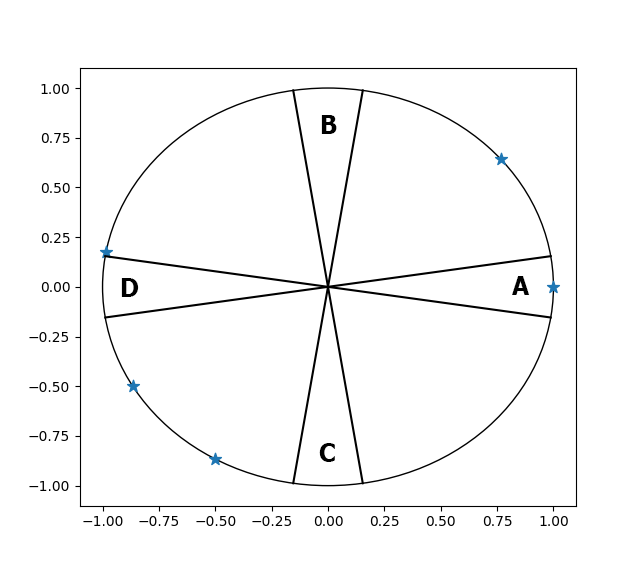
\includegraphics[scale=0.5]{initial position}

On sépare ensuite le cercle en différents cônes d'angle $\alpha$ nommés $A$, $B$, $C$, et $D$. C'est en effet ce $\alpha$ qui apparaîtra dans la formule finale. On notera $|X|$ le nombre de point dans le cône $X$ et nous ferons des disjonctions de cas sur ces derniers.

Soit $P$ un ensemble de point, on tourne le cercle comme prévu. Pour l'exemple, on positionnera les points sur le cercle mais les chemins utilisés marcheront quelque soit leur positionnement tant que l'enveloppe convexe est de la taille prévue.

\subsubsection*{1er cas} $\exists X, |X| \geq 2$

Dans ce cas, en réveillant les deux robots dans le cône avec celui initial, on peut aller réveiller les trois derniers où qu'ils soient dans le cercle. Réveiller les robots dans un cône d'angle $\alpha$ prend au plus un temps $1 + chord(\alpha)$ ce qui est montré dans d'autres papiers de recherche.
On peut donc réveiller tout le monde avec $\gamma(P) \leq 1 + chord(\alpha) + 2 = 3 + chord(\alpha)$
Notons que cette preuve s'applique dès que deux points sont sur un cône de taille $\alpha$ commun. On peut donc supposer désormais que cette situation n'arrive plus.

\subsubsection*{2ème cas} $|D| = 0$

On prend $T$ l'arbre commençant au noeud de $A$ et explorant de part et d'autre de son axe en commençant par le noeud le plus proche.
Soit $P'$ l'ensemble de point sur le cercle où les deux points des demi cercles sont répartis entre $A$ et $D$.
On a $\gamma(P) \leq  \gamma(T, P) \leq \gamma(T, P')$

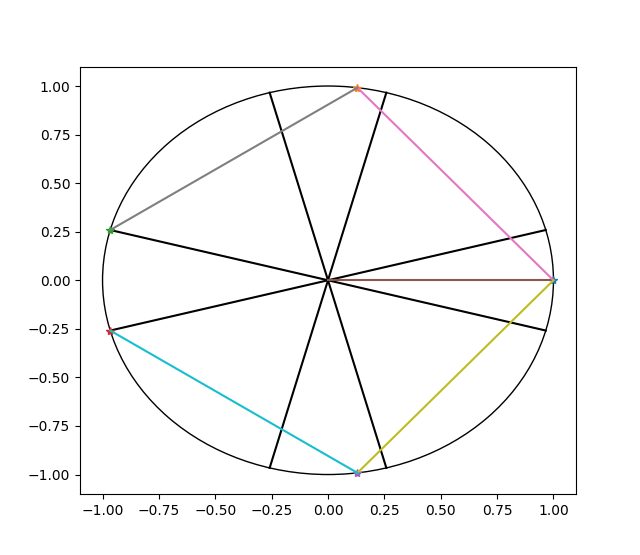
\includegraphics[scale=0.5]{2eme cas}

En effet, d'après \ref{worstchord} le pire cas pour $P$ est d'avoir un point le plus loin possible de A et d'avoir des arcs égaux, positionnant donc le dernier point du demi-cercle pile entre le point de $A$ et celui collant $D$. On a alors

$\gamma(P) \leq \gamma(T, P') = 1 + 2chord(\frac{\pi}{2} - \frac{\alpha}{4})$

\subsubsection*{3ème cas} $|B| = |C| = 0$ ($|A| = 1$ et $|D| = 1$)
Par symétrie, on peut considérer que le point dans $D$ appartient au demi-cercle du haut et donc que l'on a un seul point en haut qui ne soit pas dans $D$ que l'on nommera $b$.

\begin{itemize}

\item Si $b$ est entre $A$ et $B$

\begin{itemize}

\item si $b$ entre $A$ et $B$ et en bas 1 point de chaque côté

on choisit pour T l'arbre commençant en bas à gauche et séparant le travail des robots en 2 comme avant.
On prend ensuite le pire cas possible pour ce T.

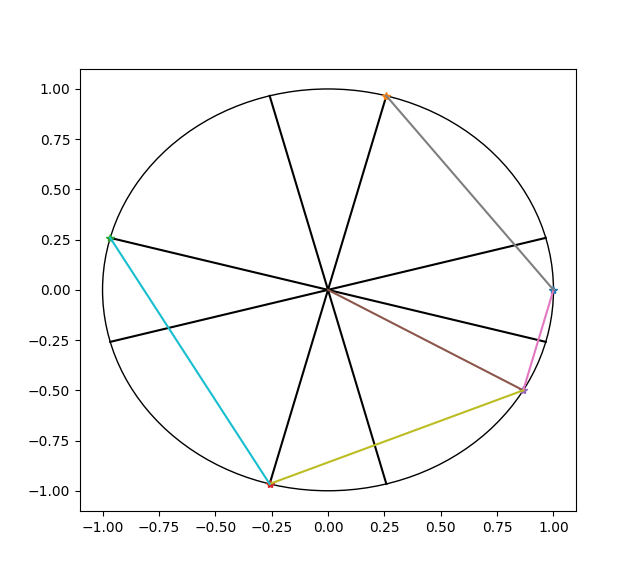
\includegraphics[scale=0.45]{3eme cas1}

En oubliant pas que l'angle entre $a$ et le point en bas à gauche est d'au moins $\alpha$ on peut donc appliquer le lemme \ref{worstchord} afin de conclure
$\gamma(P) \leq 1 + 2chord(\frac{\pi}{2} - \frac{\alpha}{4})$

\item si $b$ entre $A$ et $B$ et deux points entre $C$ et $D$
l'arbre est le suivant:

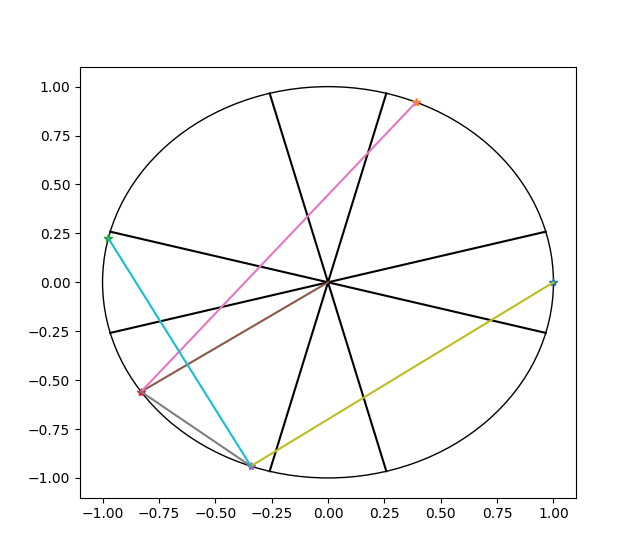
\includegraphics[scale=0.45]{3eme cas2}

Ici on néglige la branche rose car elle a une longueur totale de 3 (ce sera aussi fait dans les cas suivants)
La longueur de la branche bleue est ici $\leq 1+chord\left(\frac{\pi}{2} - \alpha\right)+chord(\frac{\pi}{2}) \leq 1 + 2chord(\frac{\pi}{2} - \frac{\alpha}{4})$
Et pour la dernière branche, on applique \ref{worstchord} pour obtenir cette borne exacte

$=> \gamma(P) \leq 1 + 2chord(\frac{\pi}{2} - \frac{\alpha}{4})$

\item Si $b$ entre $A$ et $B$ et deux points entre $A$ et $C$ on applique le même arbre

\end{itemize}

\item Si $b$ est entre $C$ et $D$

\begin{itemize}

\item Le seul cas difficile est celui où les deux points du bas sont entre $A$ et $C$.
suivant l'arbre suivant:

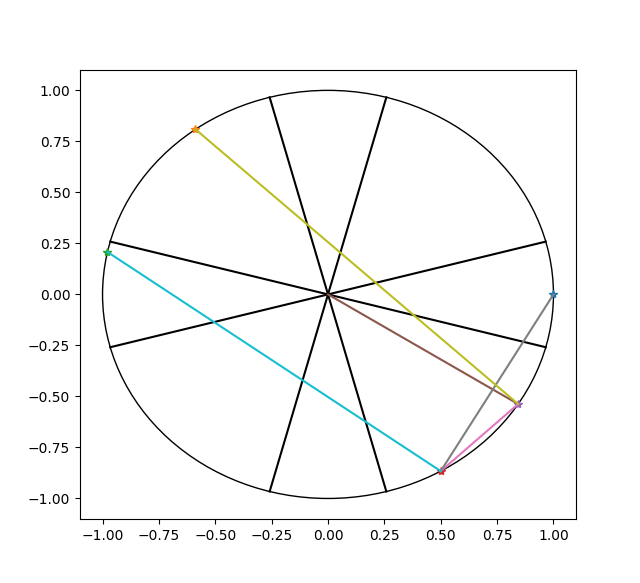
\includegraphics[scale=0.45]{3eme cas3}

La branche bleue ici se résout encore une fois par \ref{worstchord}
La branche jaune est négligée
et la branche violette permet le calcul de son pire cas en maximisant la longueur des cordes en respectant les contraintes angulaires. (en particulier que l'angle entre deux points doit être d'au moins $\alpha$)

on obtient alors
\begin{align*}
\gamma(P) &\leq max\left(1+2chord\left(\frac{\pi}{2} - \frac{\alpha}{4}\right), 1 + chord\left(\frac{\pi}{2} - \frac{3\alpha}{2}\right) + chord\left(\frac{\pi}{2} - \frac{\alpha}{2}\right)\right) \\
&\leq 1+2chord\left(\frac{\pi}{2} - \frac{\alpha}{4}\right)
\end{align*}

\item Si l'on a 2 points entre $C$ et $D$, alors on peut effectuer l'arbre suivant

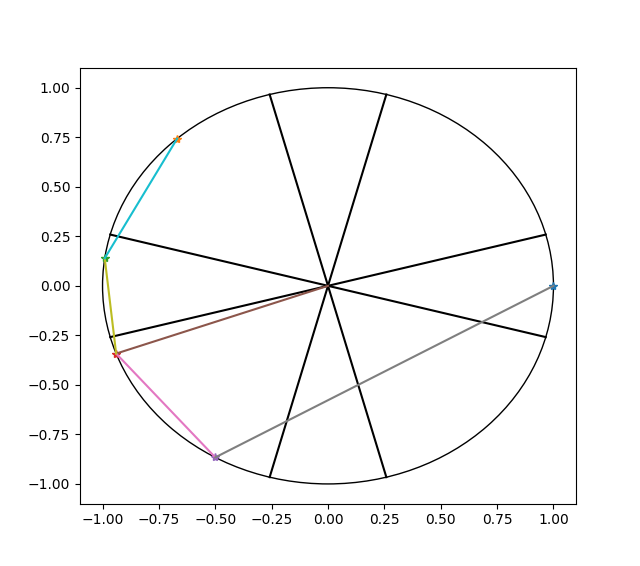
\includegraphics[scale=0.4]{3eme cas4}

On peut alors comme d'habitude utiliser \ref{worstchord} pour conclure

\item Pour dernier cas, nous avons 1 point de part et d'autre de la vertical en bas alors par un chemin similaire au point précédent:

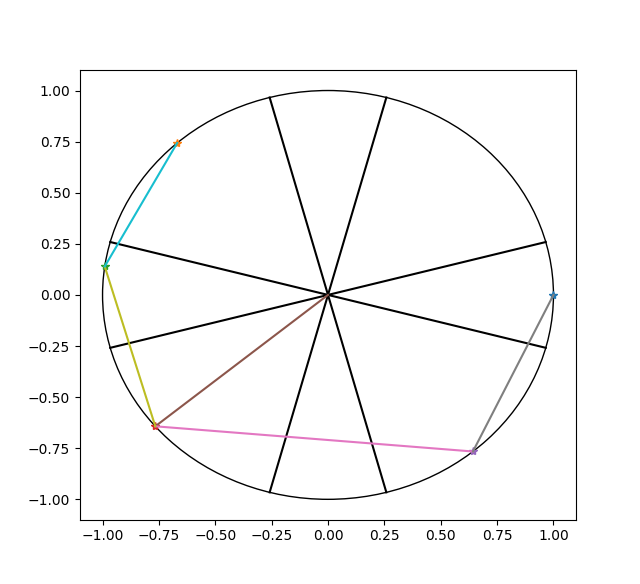
\includegraphics[scale=0.4]{3eme cas5}

Comme la dernière fois \ref{worstchord} nous permet de conclure

\end{itemize}
\end{itemize}

\subsubsection*{4eme cas} $|A| = |B| = |C| = |D| = 1$

il reste donc un 5eme point à placer qui se trouve dans un des cônes diagonaux.

\begin{itemize}

\item si il est dans un cône d'angle $\alpha$ au centre du cône diagonal.

on a alors le chemin standard commençant par le 5ème point qui nous donne par \ref{worstchord}: $\gamma(P) \leq 1 + 2chord(\frac{\pi}{2} - \frac{\alpha}{4})$

\item si ca n'est pas le cas alors on prend l'arbre commençant en ce 5 ème point mais allant vers le point le plus proche et le plus éloigné ainsi

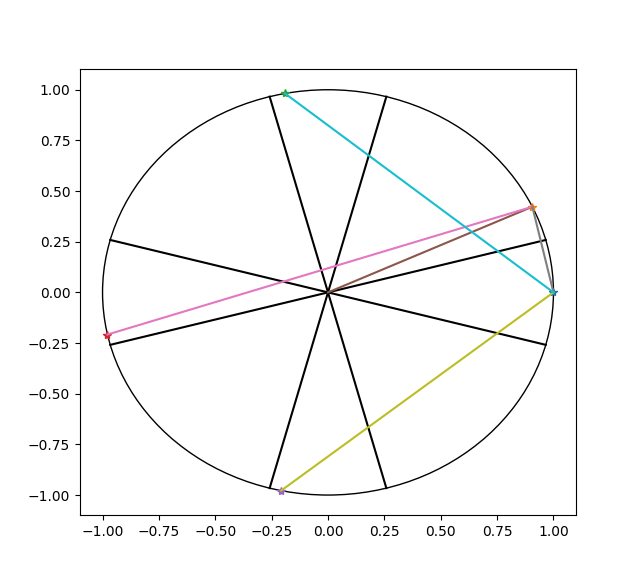
\includegraphics[scale=0.5]{4eme cas}

La branche rose est négligée
la branche bleue est a sa première partie bornée par une corde de taille $\frac{\pi}{4}$ car le point du milieu est en dessous de la ligne diagonal d'un angle au moins $\frac{\alpha}{2}$ et la deuxième partie par $\frac{\pi}{2} + \alpha$
la branche jaune est symétrique à la branche bleue.

on a donc $\gamma(P) \leq 1 + chord(\frac{\pi}{4}) + chord(\frac{\pi}{2} + \alpha) \leq max(3 + chord(\alpha), 1 + 2chord(\frac{\pi}{2} - \frac{\alpha}{4}))$

\end{itemize}

\subsubsection*{5ème cas} $|B| = |A| = |D| = 1, |C| = 0$
à noter que par symétrie, ca s'applique pour $|B| = 0$ et $|C| = 1$

\begin{itemize}

\item Si le point dans D appartient au demi-cercle du haut:

\begin{itemize}

\item Si en bas il y a un point de chaque côté, on choisit le point en bas qui se trouve du côté de B et on termine de façon standard. On a alors $\gamma(P) \leq 1 + 2chord(\frac{\pi}{2} - \frac{\alpha}{4})$

\item si en bas on a les deux points du même côté, on commence par celui au milieu des deux points qui le collent pour obtenir le même résultat.
Dans le cas où les deux points sont entre C et D on a donc

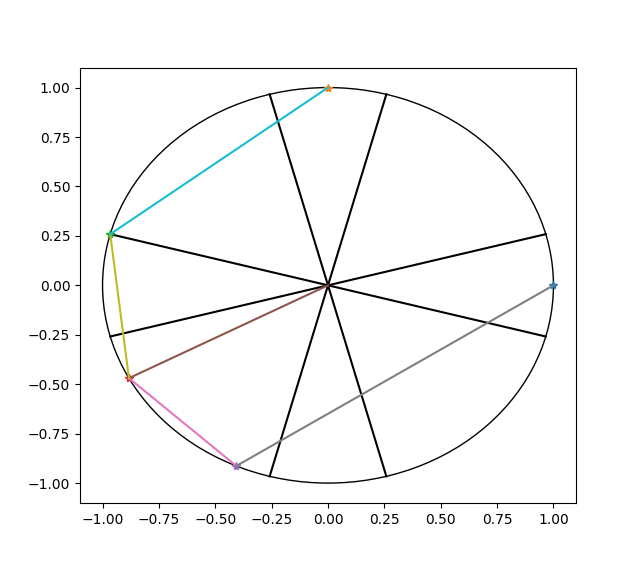
\includegraphics[scale=0.4]{5eme cas1}

Nous sommes ici encore en capacité d'utiliser \ref{worstchord}

Dans le cas où les deux sont entre A et C on a

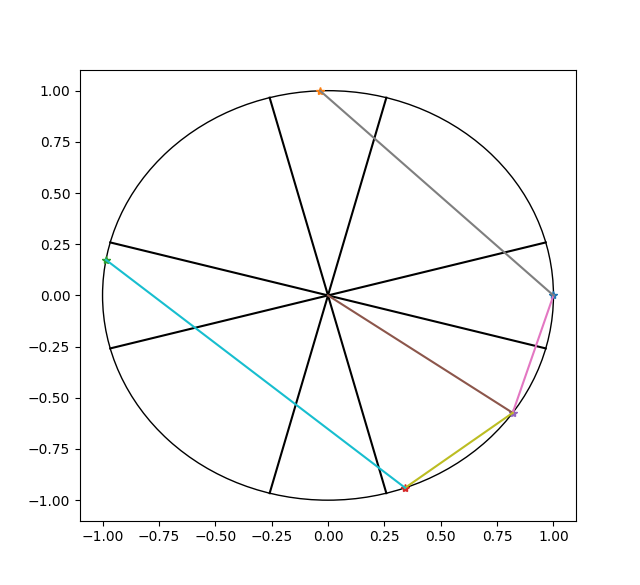
\includegraphics[scale=0.4]{5eme cas1bis}

grâce à l'écart d'angle entre les points, on a bien encore une fois les conditions d'applications de \ref{worstchord}

\end{itemize}

\item Si le point dans D appartient au demi-cercle du bas, on a 4 cas

\begin{itemize}

\item si point libre du haut entre A et B et point du bas entre A et C

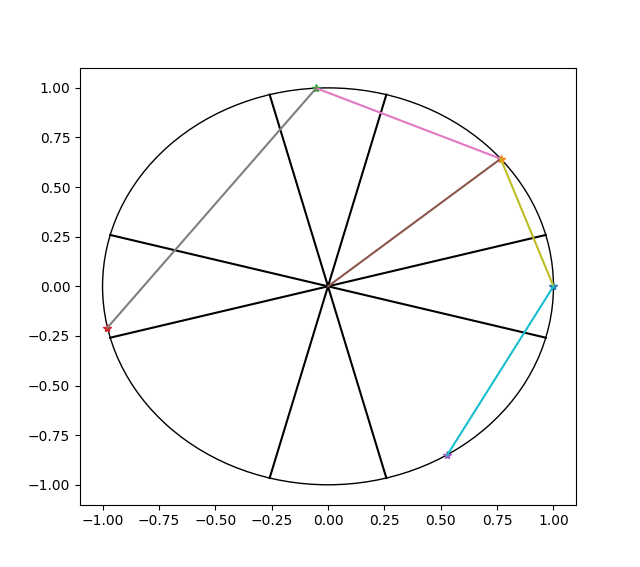
\includegraphics[scale=0.4]{5eme cas2}

en oubliant pas que le point de départ est forcément éloigné d'un angle $\alpha$ de $a$ on a bien le résultat par \ref{worstchord}

\item si point libre du haut entre A et B et point du bas entre C et D alors cela dépend de $b$. Si $b$ est sur le côté droit, on commence effectue cet arbre:

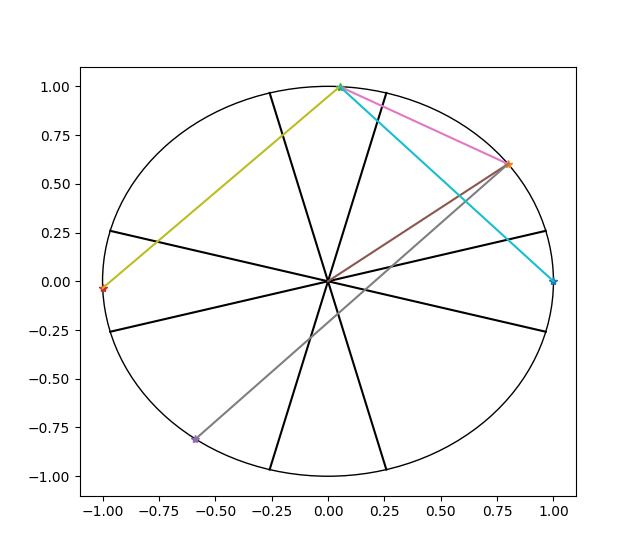
\includegraphics[scale=0.4]{5eme cas3}

on a alors

$\gamma(P) \leq max\left(1+2chord\left(\frac{\pi}{2} - \frac{\alpha}{4}\right), 1 + chord\left(\frac{\pi}{2} - \alpha\right) + chord\left(\frac{\pi}{2}\right)\right) \leq 1+2chord\left(\frac{\pi}{2} - \frac{\alpha}{4}\right)$

si maintenant $b$ est sur le côté gauche, on peut commencer par $b$. On effectuant un arbre classique, le côté gauche a la bonne borne et le côté droit est facile

\item si point libre du haut entre B et D et point libre du bas entre C et D on a l'arbre suivant.

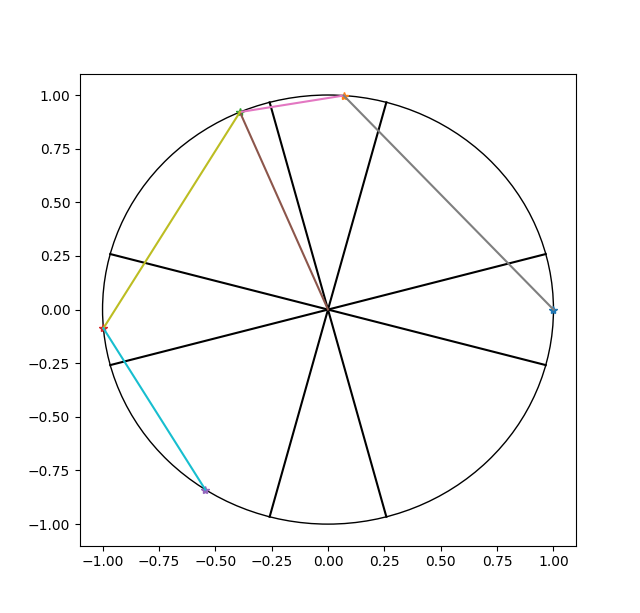
\includegraphics[scale=0.4]{5eme cas4}

\item si point libre du haut entre B et D et point libre du bas entre A et C cela dépend à nouveau de $b$. Si $b$ à droite on a (en allant vers le point le plus proche):

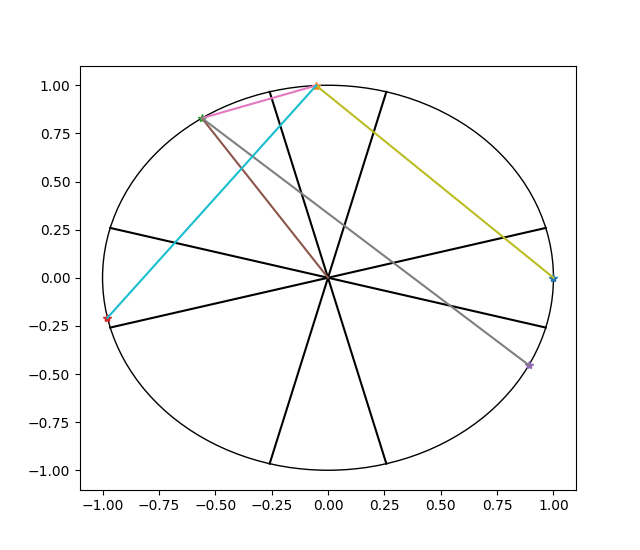
\includegraphics[scale=0.4]{5eme cas5}

en effet, on obtient alors en allant vers le plus proche que la longueur de la branche qui effectue le croisement est plus petite que $1+chord\left(\frac{\frac{\pi}{2} + \frac{\alpha}{2}}{2}\right) + chord\left(\frac{\pi}{4} + \frac{\alpha}{4}\right)$ or cette valeur est inférieure à $max\left(3 + chord\left(\alpha\right), 1 + 2chord\left(\frac{\pi}{2} - \frac{\alpha}{4}\right)\right)$ on a alors le résultat souhaité.

cependant si $b$ est à gauche on peut alors commencer par $b$ pour finir le problème comme la dernière fois.

\end{itemize}
\end{itemize}

\subsection{convexe de taille 4 ou 3}

Désormais, il faut terminer avec les cas où l'enveloppe convexe est de taille 3 ou 4. Heureusement, ces cas sont plus simples.
Si l'enveloppe convexe est de taille 3, on va vers le point le plus proche du centre qui soit à l'intérieur de l'enveloppe convexe, ensuite un des deux robots ira chercher le deuxième point à l'intérieur tandis que le deuxième ira réveiller le point le plus proche du triangle avant d'aller sur les deux autres.

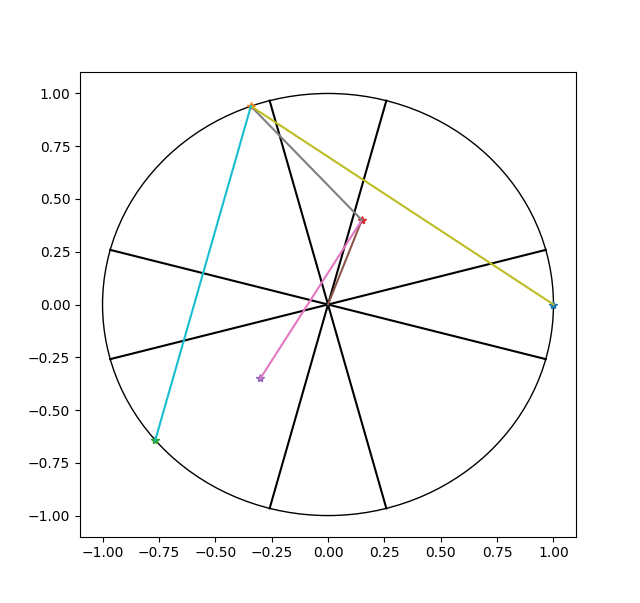
\includegraphics[scale=0.5]{n3}

En effet, le pire cas est si le point que l'on rejoint en premier est projeté sur l'enveloppe convexe orthogonalement ce qui nous donne $\exists \theta, \gamma(P) \leq \cos(\theta) + \sin(\theta) + 2 \leq \sqrt{2} + 2 \leq max(3 + chord(\alpha), 1 + 2chord(\frac{\pi}{2} - \frac{\alpha}{4}))$

Note: En réalité, cela fonctionne quelque soit l'emplacement du deuxième point à l'intérieur, et donc également si il n'est pas dans l'enveloppe connexe, et il est donc possible de traiter par exactement la même méthode le cas où l'enveloppe convexe est de taille 4.

Ainsi, on a montré le résultat voulu et par une analyse graphique, on obtient $\alpha$ tel que $\gamma(P)$ soit minimal. L'équation ne se résolvant pas facilement, on approxime et augmente la valeur pour obtenir \(\alpha_5 < 3.603564775\)